%%% Template originaly created by Karol Kozioł (mail@karol-koziol.net) and modified for ShareLaTeX use

\documentclass[a4paper,11pt,fleqn]{article}

\usepackage[T1]{fontenc}
\usepackage[utf8]{inputenc}
\usepackage{graphicx}
\usepackage{xcolor}

\usepackage{tgtermes}

\usepackage[
pdftitle={CMPS 242-HM2}, 
pdfauthor={jianfeng},
colorlinks=true,linkcolor=blue,urlcolor=blue,citecolor=blue,bookmarks=true,
bookmarksopenlevel=2]{hyperref}
\usepackage{amsmath,amssymb,amsthm,textcomp}
\usepackage{enumerate}
\usepackage{multicol}
\usepackage{tikz}

\usepackage{geometry}
\geometry{total={210mm,297mm},
left=25mm,right=25mm,%
bindingoffset=0mm, top=20mm,bottom=20mm}


\linespread{1.3}

\newcommand{\linia}{\rule{\linewidth}{0.5pt}}

% custom theorems if needed
\newtheoremstyle{mytheor}
    {1ex}{1ex}{\normalfont}{0pt}{\scshape}{.}{1ex}
    {{\thmname{#1 }}{\thmnumber{#2}}{\thmnote{ (#3)}}}

\theoremstyle{mytheor}
\newtheorem{defi}{Definition}

% my own titles
\makeatletter
\renewcommand{\maketitle}{
\begin{center}
\vspace{2ex}
{\huge \textsc{\@title}}
\vspace{1ex}
\\
\linia\\
\@author \hfill \@date
\vspace{4ex}
\end{center}
}
\makeatother
%%%

% custom footers and headers
\usepackage{fancyhdr,lastpage}
\pagestyle{fancy}
\lhead{}
\chead{}
\rhead{}
\lfoot{JIANFENG ZHAO}
\cfoot{ \thepage}
\rfoot{HM1}
\renewcommand{\headrulewidth}{0pt}
\renewcommand{\footrulewidth}{0pt}
%

%%%----------%%%----------%%%----------%%%----------%%%

\begin{document}

\title{CMPE202 -- HM1}

\author{NAME: Jianfeng Zhao, Email: jzhao65@ucsc.edu}

\maketitle



\section*{Qustion 1}



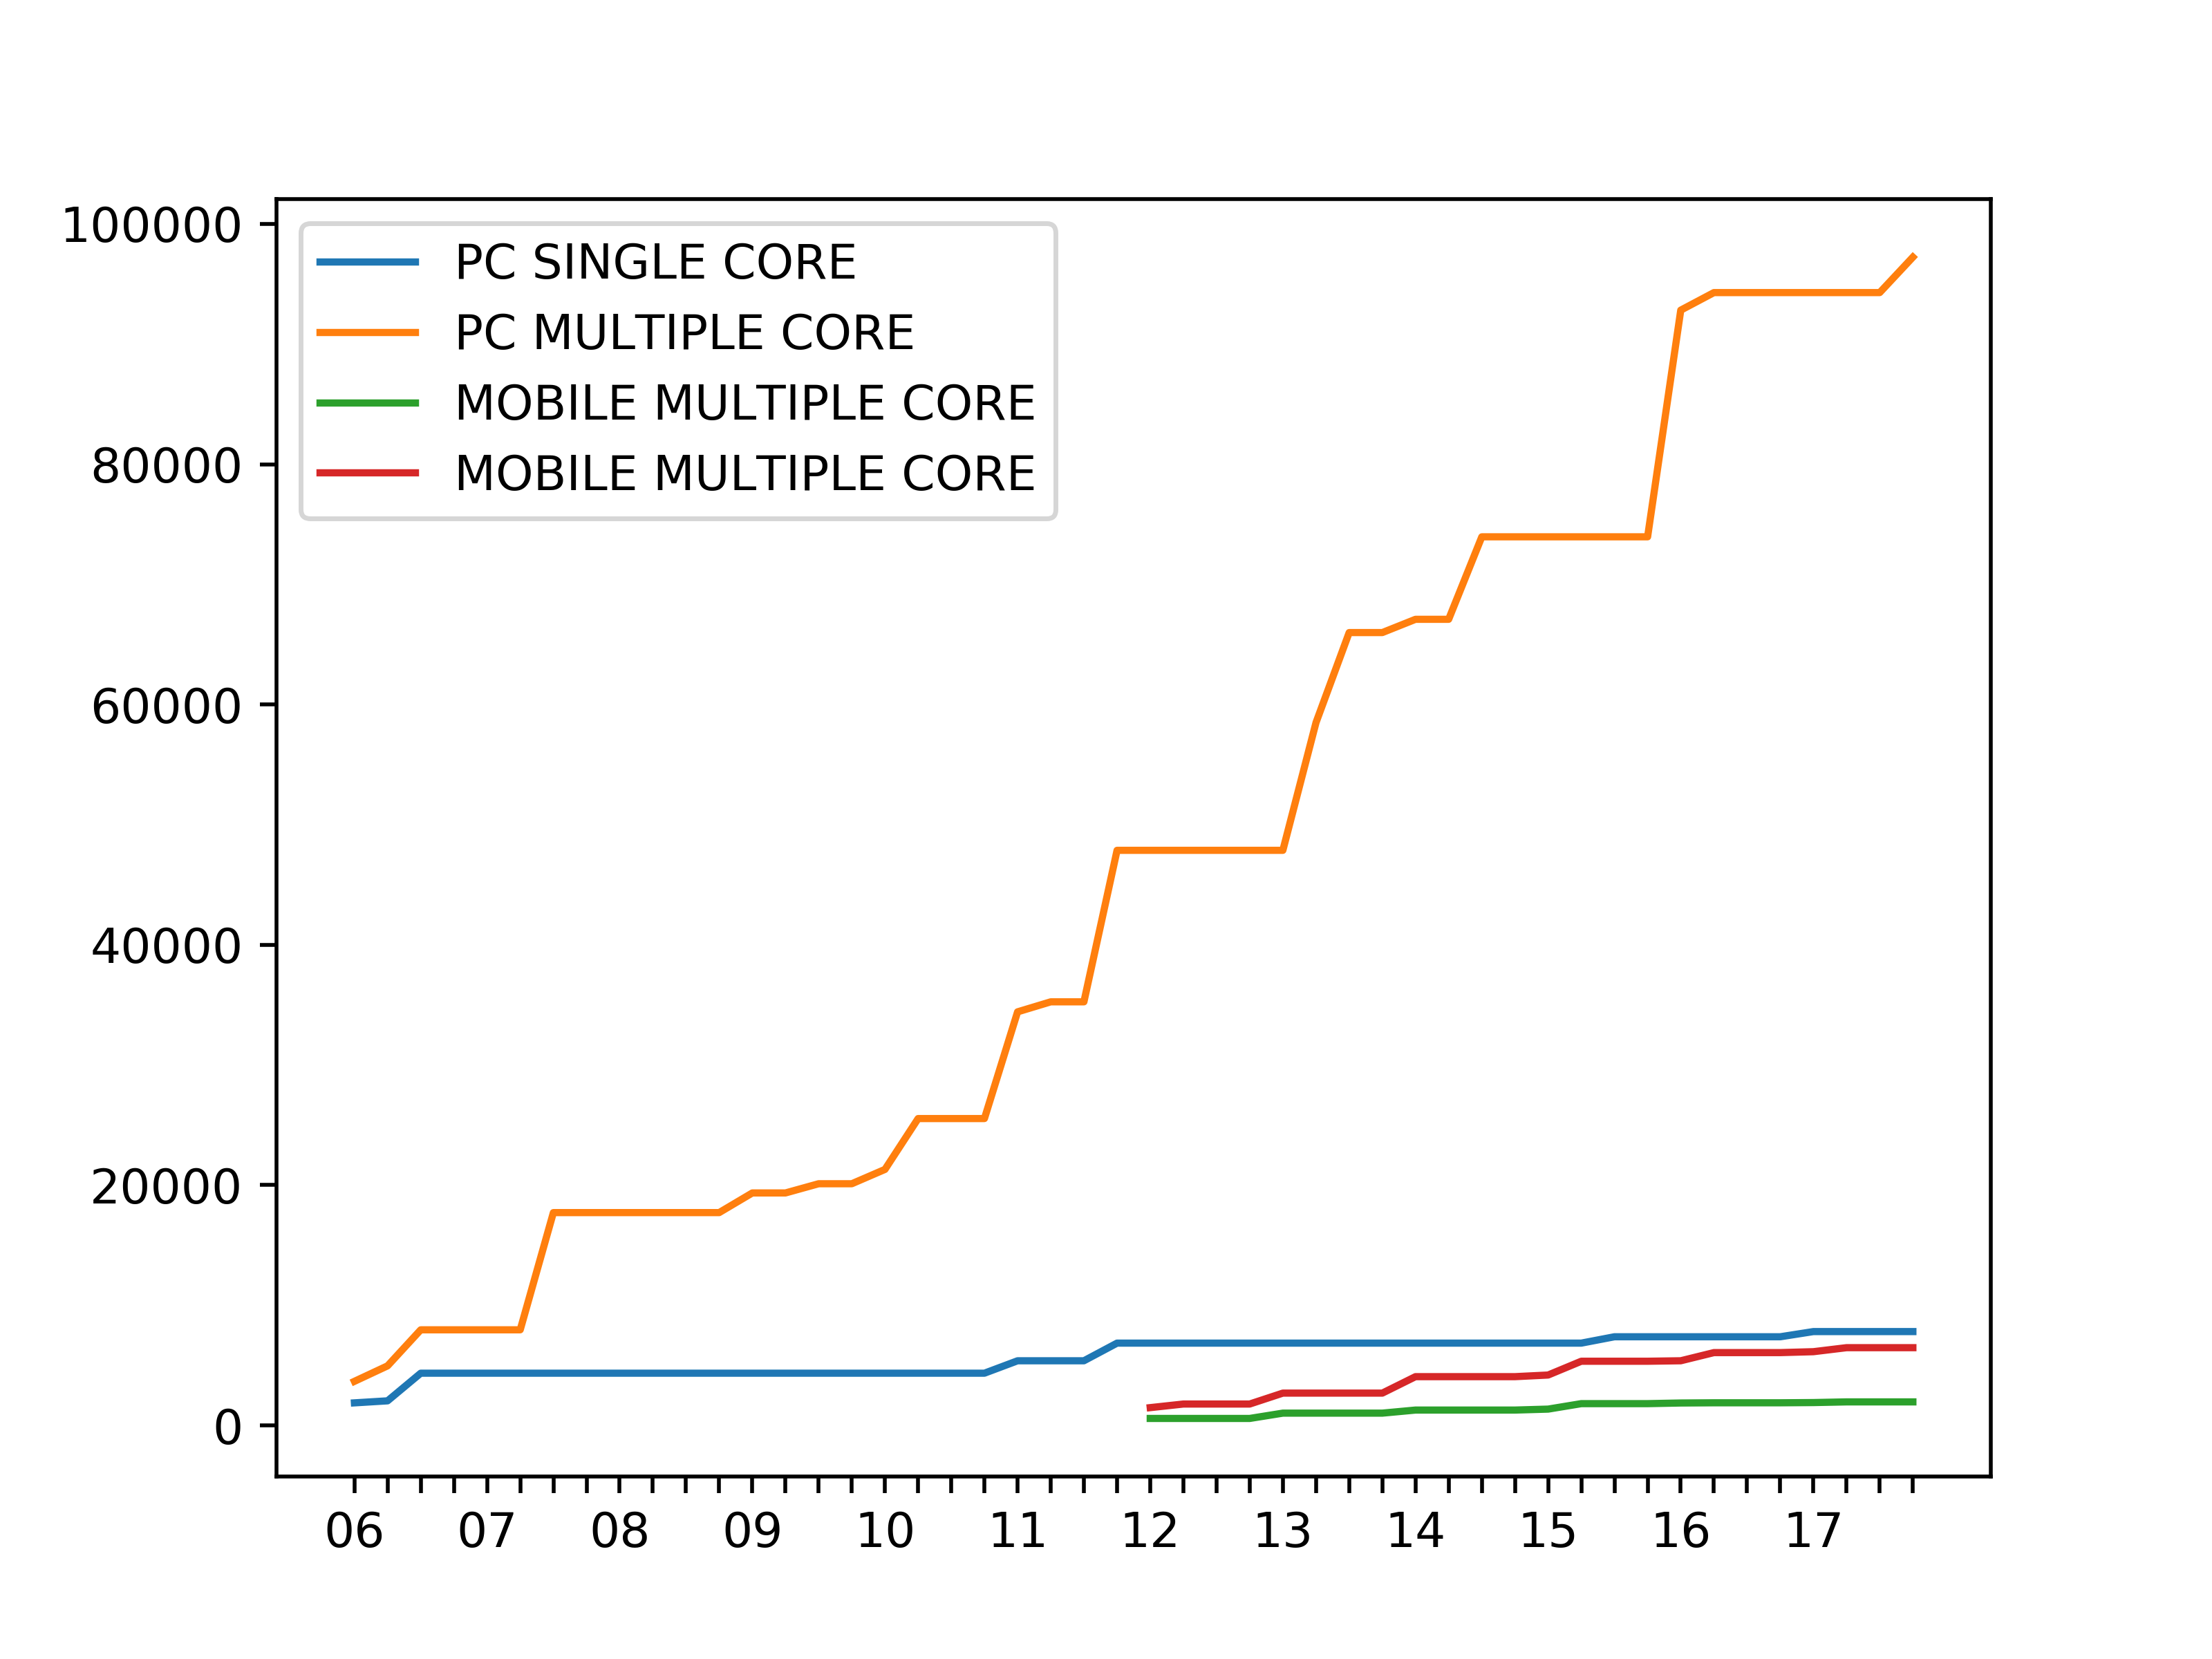
\includegraphics{plot}

\section*{Question 2}
\subsection*{2.1}
According to the Amdahl's Law, $f(e) = 0.25$, $Speedup(e) = 20$, hence, the over all speedup is:
\begin{equation}
\begin{split}
Speedup_{all} &= \frac{1}{(1 - f(e)) + \frac{f(e)}{Speedup(e)}}\\
&=\frac{1}{(1 - 0.25) + \frac{0.25}{20}}\\
&=\frac{80}{61}
\nonumber
\end{split}
\end{equation}

\subsection*{2.2}
According to Amdahl's Law, the maximum possible theoretical speedup is:
\begin{equation}
Max Speedup = \frac{1}{1 - f(x)}
\nonumber
\end{equation}
According the the question, $f(x) = 0.4$ , Hence, 
\begin{equation}
Max Speedup = \frac{1}{1 - 0.4} =\frac{5}{3}
\nonumber
\end{equation}

\subsection*{2.3}
According to the question, $Speedup_{gpu\_cpu} = \frac{80}{61}$ and Vector can improve 20\% code which means $f(e) = 0.2$, Hence, According to Amdahl's Law:
\begin{equation}
Speedup_{max} = \frac{1}{1 - f(x)} = \frac{5}{4} = 1.25
\nonumber
\end{equation}
But $Speedup_{gpu\_cpu} = \frac{80}{61} = 1.31$, which is greater than 1.25. Which means this configuration will never reach the configuration of GPU-CPU configuration.\\
Hence,  Vector to match the overall speedup of the GPU+CPU configuration in the part one  is impossible.

\section*{Question 3}
According to the question, instruction run like below:\\
\begin{tabular}{|p{3pt}|  p{15pt}  p{35pt}  | p{3pt} p{3pt} p{3pt} p{3pt} p{3pt} p{3pt} p{3pt} p{3pt} p{3pt} p{3pt} p{3pt} p{3pt} p{3pt} p{3pt} p{3pt} p{3pt} p{3pt} p{3pt} p{3pt} p{3pt} p{3pt} p{3pt} p{3pt} p{3pt}p{1pt}|}
\hline 
1&add & a3,a5,32 &F0&F1&D0&X0&W0&&&&&&&&&&&&&&&&&&&&\\
\hline
2&lw  & a4,0(a5) &&F0&F1&D0&X0&X1&X2&W0&&&&&&&&&&&&&&&&&\\
\hline
3&addw & a1,a1,a4&&&F0&F1&D0&D0&D0&X0&W0&&&&&&&&&&&&&&&&\\
\hline
4&add&a5,a5,4&&&&F0&F1&F1&F1&D0&X0&W0&&&&&&&&&&&&&&&\\
\hline
5&bne&a5,a3,.L2&&&&&F0&F0&F0&F1&D0&X0&W0&&&&&&&&&&&&&&\\
\hline
6&lw  & a4,0(a5)&&&&&&/&/&/&/&/&F0&F1&D0&X0&X1&X2&W0&&&&&&&&\\
\hline
7&addw & a1,a1,a4&&&&&&&&&&&&F0&F1&D0&D0&D0&X0&W0&&&&&&&\\
\hline
8&add&a5,a5,4&&&&&&&&&&&&&F0&F1&F1&F1&D0&X0&W0&&&&&&\\
\hline
9&bne&a5,a3,.L2&&&&&&&&&&&&&&F0&F0&F0&F1&D0&X0&W0&&&&&\\
\hline
10&lui&a0,\%hi(.LC1)&&&&&&&&&&&&&&&/&/&/&/&/&F0&F1&D0&X0&W0&\\
\hline
\end{tabular}
\\
\\
Because Load instruction need to takes 3 cycle. Line 2 need 3 cycles to excute load word.\\
Also, this data hazerd can be solute by data forwarding. Hence, line 3 need to wait in Instruction Decode for 2 cycles. line 4, 5 also need to wait 2 cycles in F1 and F0 individually.\\
As well as RISCV ISA don't have delay slot, therefor, in line 6, CPU must stall for 5 cycles to wait the answer of instruction BNE. \\
BNE will one taken instruction. So, we loop one time. \\
\\
Finally, cycle of every instruction as below:\\

\begin{tabular}{|| l  l | l | l | l | l ||}
\hline
\multicolumn{2}{||l|}{Instruction} & F & D & X & W\\
\hline
add & a3,a5,32 &1, 3&3, 4&4, 5&5, 6\\
\hline
lw  & a4,0(a5) & 2, 4& 4, 5&5, 8&8, 9\\
\hline
addw & a1,a1,a4& 3, 5&5, 8&8, 9& 9, 10\\
\hline
add&a5,a5,4&4, 8&8, 9&9, 10&10, 11\\
\hline
bne&a5,a3,.L2&5, 9&9, 10&10, 11&11, 12\\
\hline
lw  & a4,0(a5)&11, 13&13, 14&14, 17&17, 18\\
\hline
addw & a1,a1,a4&12, 14&14, 17&17, 18&18, 19\\
\hline
add&a5,a5,4&13, 17&17, 18&18, 19&19,20\\
\hline
bne&a5,a3,.L2&14, 18&18, 19&19, 20&20, 21\\
\hline
lui&a0,\%hi(.LC1)&20, 22&22, 23&23, 24&24, 25\\
\hline
\end{tabular}

\end{document}
